\chapter{Completion in Pharo}
\label{chap:PharoCompletion}

In this chapter, we give a detailed overview of the implementation details behind the current completion engine in the Pharo IDE, challenges of code completion for a dynamically typed language, as well as describe the idea behind the sorter plugin.

\section{Code Completion Background}
\label{sec:PharoCompletion-Background}
So, first things first. The Pharo programming language is an object-oriented dynamically typed programming language with a Smalltalk-like syntax. The Pharo IDE is a programming environment meant specifically for developing in Pharo. You have a virtual machine (VM), on top of which an image can be run, which, referencing other IDEs, sort of serves as the current IDE workspace.

The interesting thing here is that the Pharo IDE itself is written in Pharo, and can be extended from within. This means that when implementing code completion, you can be testing it live in the very environment where you are developing it, which, of course, if not done carefully, can lead you to breaking the system. However, this pecularity is still an immense advantage with a project like this.

Now, code completion in the Pharo IDE is called at every keystroke, after we have typed two and more alphabetic characters. We create a completion context for all the text typed up until then, be it in the Playground or in the Editor. (Essentially, the Playground is a tool for generating small scripts and sketching out some code, whereas the Editor is where you write and edit code for a particular method of a class, i.e. the place to implement the functionality of your classes; Fig. \ref{fig:playground} and \ref{fig:editor}).

\section{Typing for Completion in Dynamic Languages}
\label{sec:PharoCompletion-Typing}
As Pharo is a dynamically typed language, the precise type information is only available at runtime. This is of course tricky for code completion, because the type is not known at the moment of typing, which can make the completion suggestions for message sends appear too general. This is ineffective, as often the specific completion the developer has in mind can be too far down the list of suggestions and it would require scrolling through the suggestions list, or typing more characters.

There are a couple of approaches one could take to solve this. The first is type inference (or rather type reconstruction), which can be done by extracting interface types by looking at the messages sent to a variable, and merging these results with types found by heuristics working on right-hand side of assignment expressions (\cite{Pluq09a}). Type guessing by means of name analysis can also be done, but is more likely to be misleading. The third approach, which is the one taken with the AST-based completion in the Pharo IDE (more details in the next section), involves performing a semantic analysis of source code, which allows to get accurate type information for certain kinds of nodes.

\begin{figure}[H]
    \centering
    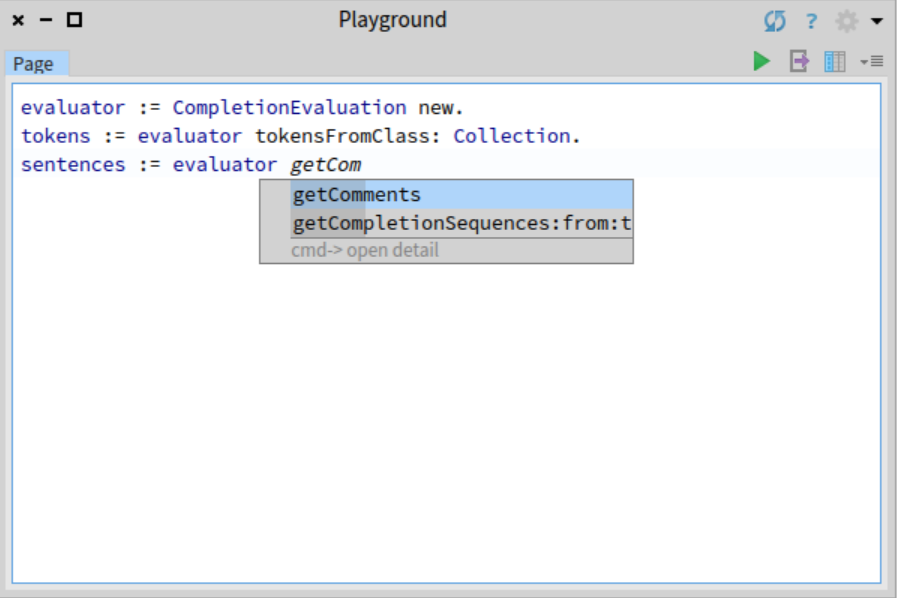
\includegraphics[width=0.9\linewidth]{images/completion1.png}
    \caption{Completion in the Playground}
    \label{fig:playground}
\end{figure}

\begin{figure}[H]
    \centering
    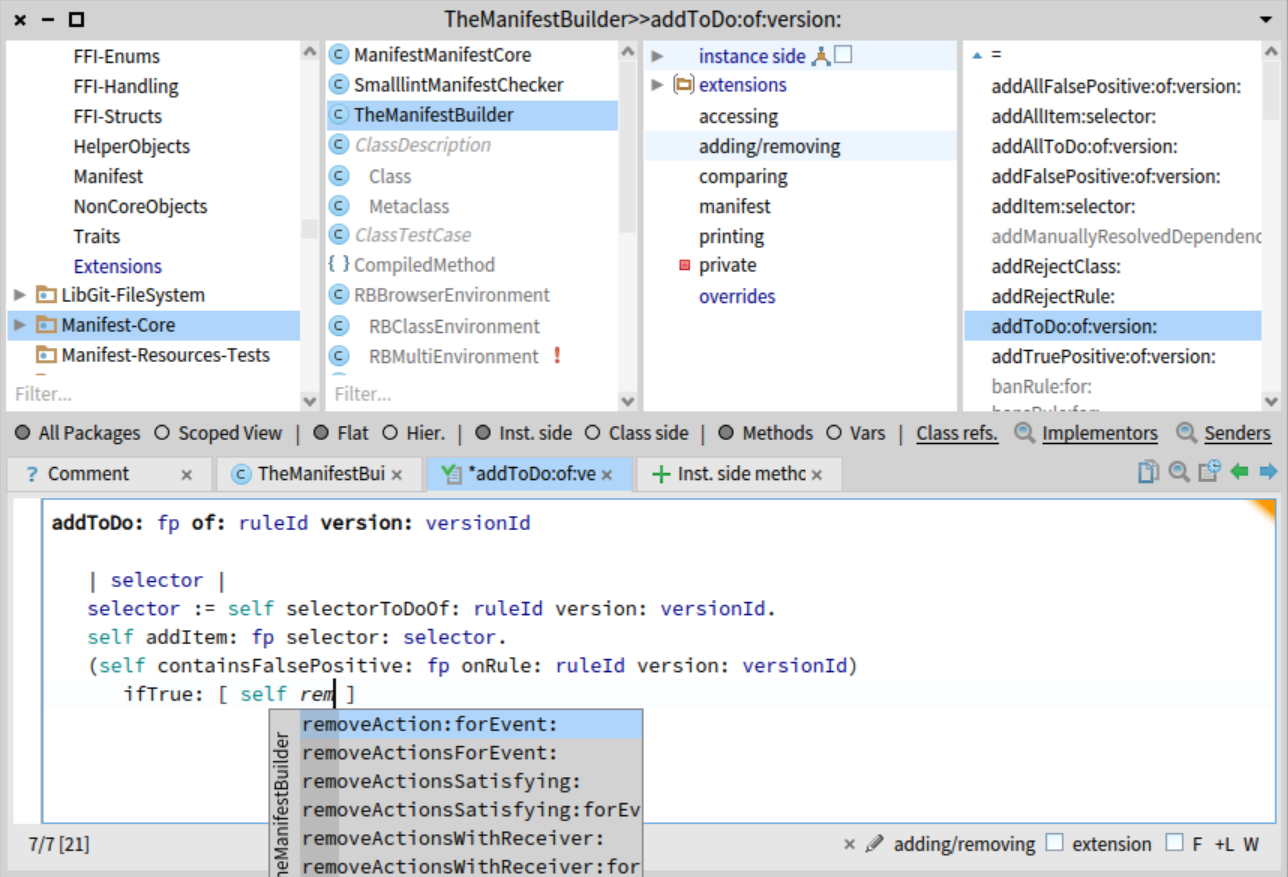
\includegraphics[width=0.9\linewidth]{images/completion2.png}
    \caption{Completion in the Editor}
    \label{fig:editor}
\end{figure}

\section{AST-Based Completion}
\label{sec:PharoCompletion-ASTCompletion}
The approach behind implementing the AST-based completion is as follows:

The completion context parses the text and transforms it into the AST representation, such as a sequence of AST nodes. In the process all the information needed for further actions is extracted: for example, we get the currect position of the cursor (i.e. where we want to get the completion) and the class where we are currently operating (or information that it's in the Playground). Doing the semantic analysis, we get the most fitting type of node for each part of code, and then go to each node to get the correct completion behaviour. For instance, this means that for a Global node, we want to be suggested all the globals, such as class names, for a Message node we only want to get message sends to a variable (in other words, method calls applicable to a certain class instance), and so on.

Combining the available symbol prefix of length 2 and more that we have, as well as relevant semantic information, we are able to give a list of fitting completion suggestions that are then passed to the sorter and, in the default Pharo IDE completion, are sorted alphabetically. The list itself is displayed in a completion menu that pops up once the completion is called and then is updated with every new keystroke, unless the developer cancels it by pressing \textit{Esc} or clicking to the side of the text area. The completion window can also disappear once there are no valid suggestions to give anymore.

As has been mentioned above, generally alphabetically sorted completions can be quite inaccurate for variables and method sends of an unknown type. There is, however, one silver lining: to have a sorting strategy that would suggest more contextually relevant results first, and in such a way compensate for a lack of typing precision. For this, we implemented a sorter plugin.

\section{Sorter Plugin}
\label{sec:PharoCompletion-SorterPlugin}
The sorter plugin is technically a part of the completion but it's implemented separately and is intended for usage even without knowing the details of the completion engine. Specifically, within the sorter we treat the completion implementation as a sort of a black box, and the only information we receive is the list of completions we want to sort, as well as the context. This was done to make the sorter extendable and open for modication by any developer, so one could take the general completion functionality and then on top of it put any sorting strategy they would like to have.

Essentially, this means that the way we get the completion results themselves is the same, i.e. we semantically analyse the source code and try to give relevant nodes as precisely as possible. However, the sorting strategy really matters when it comes to tokens where we cannot give any precise suggestions by analysis alone, and displaying them in a certain order, that the developer of the sorting strategy hypothesises to be helpful, can really improve the end result (i.e. the list of suggestions displayed in the pop up completion menu).

\section{Summary}
\label{sec:PharoCompletion-Summary}
In short, the main things to remember from this chapter are the following:
\begin{itemize}
    \item Pharo is a dynamically typed languaged based on Smalltalk, and the Pharo IDE is a programming environment specifically for developing in Pharo
    \item code completion in the Pharo IDE is used in two places: the Playground (a scripting tool) and the Editor (tool for writing and editing class functionality)
    \item current code completion is based on AST analysis of source code; it is called after the developer types two alphabetic characters, and the completion candidates are suggested by the most relevant semantic context
    \item there's a sorter plugin that supports implementing various sorting strategies; by default completion candidates are sorted alphabetically
\end{itemize}